I have created this demo to showcase some 3D Graph sketching with Python + Matplotlib Library. I wont explain code but consider these examples as a starting point.
Consult the web for library documentation for certain functions being used in my code samples below.

Check out https://matplotlib.org/ for more information on the Matplotlib library.

\begin{lstlisting}[language=Python]
import numpy as np 
import matplotlib.pyplot as plt 
import mpl_toolkits.mplot3d

#plot 3d planes 2x+2y+3z=0 and 3x+5y+7z=0

#increase dpi
plt.rcParams['figure.dpi'] = 200
x = np.linspace(-5,5,100)
y = np.linspace(-5,5,100)
X,Y = np.meshgrid(x,y)
Z = 2*X+2*Y+3
fig = plt.figure()
ax = fig.add_subplot(111, projection='3d')
ax.plot_surface(X,Y,Z,alpha=0.2)
Z = 3*X+5*Y+7
ax.plot_surface(X,Y,Z,alpha=0.2)
### you can add more graphs here ... following this procedure
ax.set_title('2x+2y+3z=0 and 3x+5y+7z=0')
plt.show()
\end{lstlisting}

\begin{figure}[H]
\centering
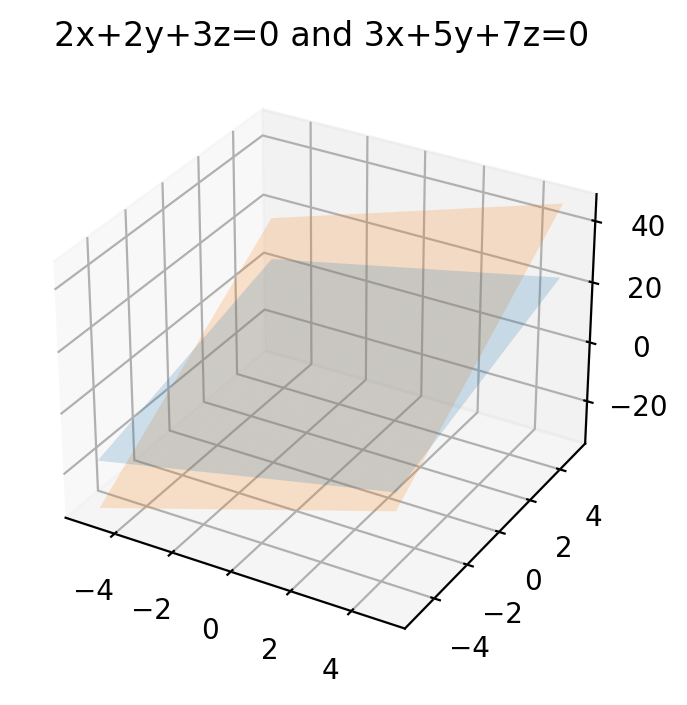
\includegraphics[width=0.5\textwidth]{output_1_0.png}
\caption{3D Graph of $2x+2y+3z=0$ and $3x+5y+7z=0$ generated with Matplotlib}
\label{fig:line3d}
\end{figure}

\begin{lstlisting}[language=Python]
import numpy as np 
import matplotlib.pyplot as plt 
import mpl_toolkits.mplot3d
#increase dpi
plt.rcParams['figure.dpi'] = 200
#plot 1/2*cos(x+y)
x = np.linspace(-5,5,100)
y = np.linspace(-5,5,100)
X,Y = np.meshgrid(x,y)
Z = 0.5*np.cos(X+Y)
fig = plt.figure()
ax = fig.add_subplot(111, projection='3d')
ax.plot_surface(X,Y,Z,alpha=0.2)
#show title
ax.set_title('1/2*cos(x+y)')
plt.show()
\end{lstlisting}    

\begin{figure}[H]
\centering
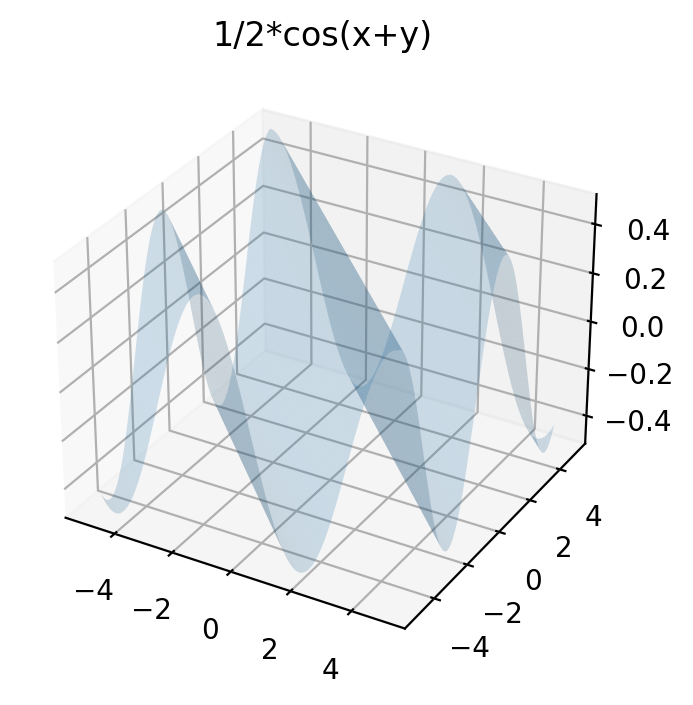
\includegraphics[width=0.5\textwidth]{output_2_0.png}
\caption{3D Graph of $\frac{1}{2}\cos(x+y)$ generated with Matplotlib}
\end{figure}

\begin{lstlisting}[language=Python]
def f(x, y):
    return np.sin(np.sqrt(x ** 2 + y ** 2))
#increase dpi
plt.rcParams['figure.dpi'] = 200
x = np.linspace(-6, 6, 50)
y = np.linspace(-6, 6, 50)
X, Y = np.meshgrid(x, y)
Z = f(X, Y)
fig = plt.figure()
ax = plt.axes(projection='3d')
ax.contour3D(X, Y, Z, 50, cmap='rainbow_r')
ax.set_xlabel('x')
ax.set_ylabel('y')
ax.set_zlabel('z')
#set title of equation
ax.set_title('sin(sqrt(x^2+y^2))')
plt.show()
\end{lstlisting}

\begin{figure}[H]
\centering
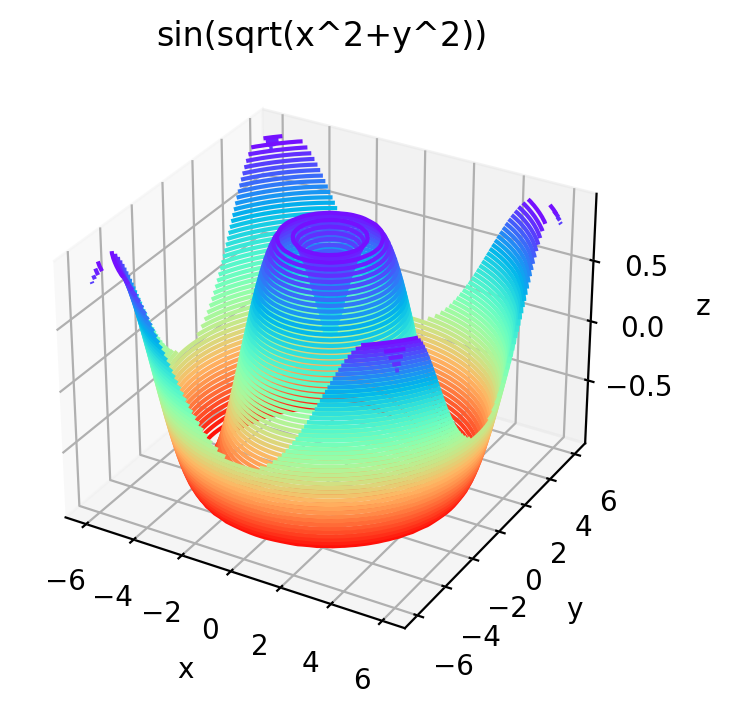
\includegraphics[width=0.5\textwidth]{output_3_0.png}
\caption{3D Graph of $\sin(\sqrt{x^2+y^2})$ generated with Matplotlib}
\end{figure}

\newpage

\begin{lstlisting}[language=Python]
import numpy as np 
import matplotlib.pyplot as plt 
import mpl_toolkits.mplot3d

#increase dpi
plt.rcParams['figure.dpi'] = 200

#plot x^2+2y+5=0 in 3d
x = np.linspace(-5,5,100)
y = np.linspace(-5,5,100)
X,Y = np.meshgrid(x,y)
Z = X**2+2*Y+5
fig = plt.figure()
ax = fig.add_subplot(111, projection='3d')
ax.contour3D(X,Y,Z,50,cmap='twilight_shifted')
#show title
ax.set_title('x^2+2y+5=0')
plt.show()
\end{lstlisting}
\begin{figure}[H]
\centering
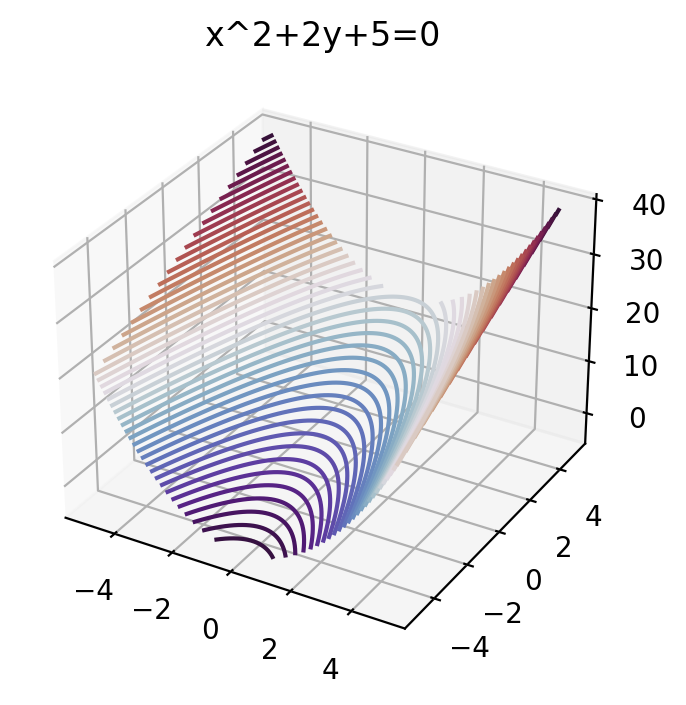
\includegraphics[width=0.5\textwidth]{output_4_0.png}
\caption{3D Graph of $x^2+2y+5=0$ generated with Matplotlib}
\end{figure}

\newpage
From manpulating my code you could easily explore and graph any function you desire. You can be creative with the colors, shapes, and sizes of the graphs.
If you want to just play around have fun! I hope you enjoy my demo and code sample.

This library is so powerful you can do anything possible with it the creativity and research is up to you.


